%%%%%%%%%%%%%%%%%%%%%%%%%%%%%%%%%%%%%%%%%%%%%%%%%%%%%%%%%%%%%%%%%%%%%%%%%%%%%%%%%%%%%%%%%%%%%%%
%                                          HYPEROPT                                           %
%%%%%%%%%%%%%%%%%%%%%%%%%%%%%%%%%%%%%%%%%%%%%%%%%%%%%%%%%%%%%%%%%%%%%%%%%%%%%%%%%%%%%%%%%%%%%%%
\chapter{Hyper-parameter Optimization of Neural Networks}
\label{chap:hyperopt}

\begin{chapabstract}
 Coucou
\end{chapabstract}

\minitoc

\newpage

%%%%%%%%%%%%%%%%%%%%%%%%%%%%%%%%%%%%%%%%%%%%%%%%%%%%%%%%%%%%%%%%%%%%%%%%%%%%%%%%%%%%%%%%%%%%%%%
\section{Defining the Problem}

The problem of hyper-parameter optimization appears when a model is governed by multiple hyper-parameters that are difficult to manually tune due to a lack of understanding in their effects. The problem gets worse when the hyper-parameters are not independent and it becomes necessary to tune them at the same time. The most intuitive solution is to test all possible combinations, but it grows exponentially with the number of hyper-parameters, making this approach usually unusable for neural networks.

In practice, as it is usually impossible to prove the optimality of a solution without testing them all, the accepted solution is the best found in the budget allocated by the user to the search.

Even though this problem appears in all kinds of situation, we are interested here in the optimization of deep learning models, as they have many hyper-parameters and we lack the understanding and the theoretical tools to tune them.

%%%%%%%%%%%%%%%%%%%%%%%%%%%%%%%%%%
\subsection{Notation}
\label{ssec:notation}

In this chapter we refer to a \textit{model} as a neural network, even though the black-box methods presented in Section~\ref{ssec:black_box} work for other machine learning models. The \textit{parameters} of a model are the weights of the network which are learned during training. The \textit{hyper-parameters} are the parameters governing the architecture of the networks (such as the number of layers or the type of layers) and the ones governing the training phase (such as the learning rate or the batch size). 

A \textit{hyper-parameter space} $\mathrm{X}$ is a hypercube where each dimension is a hyper-parameter and the boundaries of the hypercube are the boundaries of each hyper-parameter. Each point in the hyper-parameter space is referred to as a \textit{combination} $\mathrm{x} \in \mathrm{X}$. To each combination is associated a value $\mathrm{y}$ corresponding to the performance metric of the underlying neural network on the task it is trained to solve. We name $f$ a function taking as input a combination $\mathrm{x}$, build and train the underlying model and output its performance $\mathrm{y}$.

%%%%%%%%%%%%%%%%%%%%%%%%%%%%%%%%%%
\subsection{Black-box Optimization}
\label{ssec:black_box}

From the notation of Section~\ref{ssec:notation}, the goal of hyper-parameter optimization is to find the combination $\mathrm{x_*}$ minimizing the performance $\mathrm{y}$ (typically the performance is a loss function, which we want to minimize):
\begin{equation}
	\mathrm{x_*} = \argmin_{\mathrm{x} \in \mathrm{X}} f(\mathrm{x})
\end{equation}

This is the problem of hyper-parameter optimization viewed as black-box optimization. Methods in this category are independent from the model and could be used for any kind of mathematical function. However the hyper-parameters we are interested in are of a varied nature (continuous, discrete, categorical), limiting us to derivative-free optimization methods. This section is not a review of derivative-free algorithms, but an overview of the popular algorithms used specifically for hyper-parameter optimization.

Additionally, since the function $f$ is a process training a neural network, evaluating a combination is costly in time and computing resources. Moreover we have little understanding of the influence of each hyper-parameter on the performance of the model, resulting in very large boundaries and a much bigger space than needed. Worse, combinations near the boundaries of the hyper-parameter space can build a network too big to fit in the available memory, requiring us to have a way to handle evaluation failures. 

While it is tempting to simply return an extremely bad performance, this cause problems to methods assuming some structure in the hyper-parameter space. For example, a continuous hyper-parameter that gives a smooth output will suddenly have a discontinuity, and a method assuming smoothness might not work anymore. In practice, there are method-dependent solutions to this problem.

\subsubsection{Grid Search}

The most basic method is usually called \textit{grid search}. Exceedingly easy to implement, it simply test every possible combination (typically with uniform sampling for the continuous hyper-parameters). With only a handful of hyper-parameters to optimize and with a function $f$ fast to evaluate, it can be advisable to use as a first step, if only to get sensible boundaries on each hyper-parameter. 

But in the context of deep learning, hyper-parameters are too numerous, meaning there are too many combinations to evaluate, and each evaluation is costly. Also, a typical implementation in nested for-loops goes from one corner of the hyper-parameter space to the opposite corner in order. It is unlikely that the corner the search starts from happens to be an area filled with good models, since combinations in corners are extreme values of hyper-parameters and build atypical neural networks. 

Grid search can still be used with a wide enough sampling of the hyper-parameters to get an idea on where the interesting models are located and refine the boundaries, but even for that other methods are preferable.

\subsubsection{Random Search}

One step above grid search is \textit{random search}. A big limitation of grid search is that the order it goes through the hyper-parameter space is very dependent on the implementation and it always selects the same limited set of values for each hyper-parameter. Random search instead draws the value of each hyper-parameter from a uniform distribution, allowing for a much wider range of explored values.

\begin{figure}[htb]
	\begin{minipage}[b]{.49\linewidth}
		\centering
		\centerline{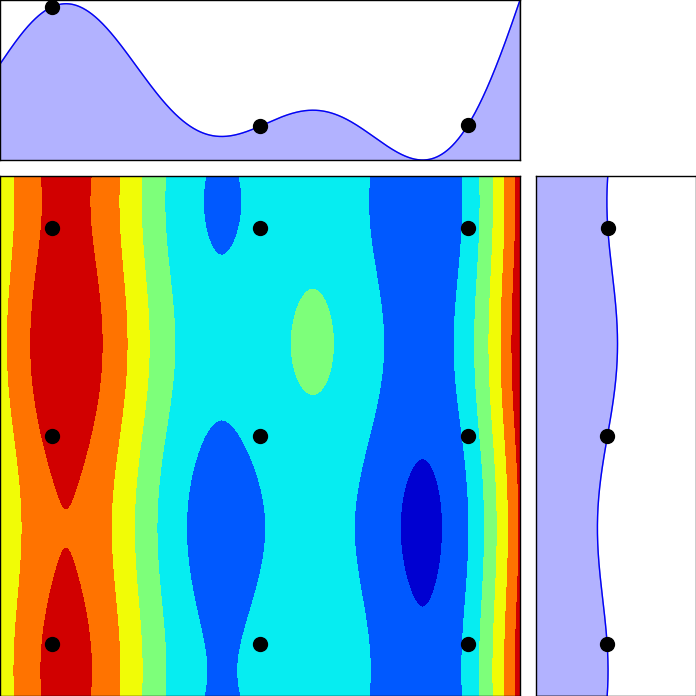
\includegraphics[width=7.2cm]{img_hyperopt/rs_grid}}
	\end{minipage}
	\begin{minipage}[b]{.49\linewidth}
		\centering
		\centerline{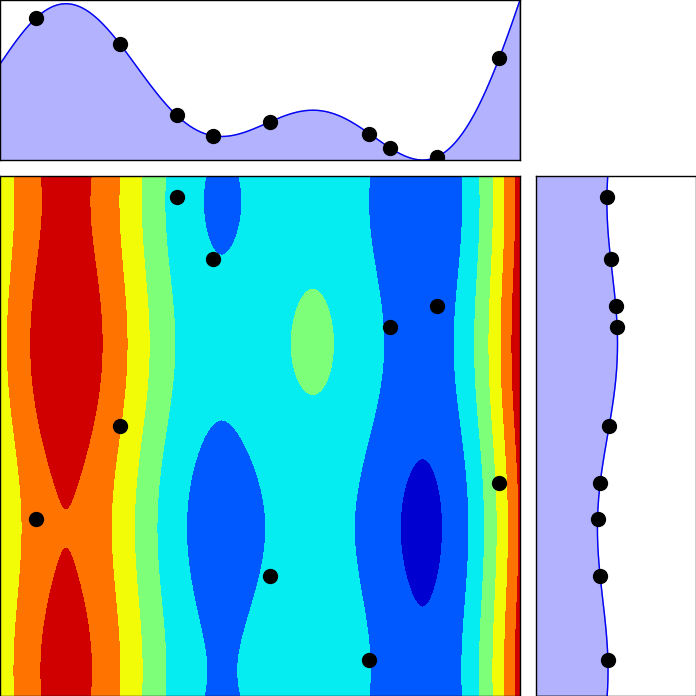
\includegraphics[width=7.2cm]{img_hyperopt/rs_random}}
	\end{minipage}
	\caption{Loss function for a two dimensional space. (Left) Grid search. (Right) Random search. At equal number of tried combinations, random search finds a better solution.}
	\label{fig:rs}
\end{figure}

Figure~\ref{fig:rs} illustrates this. Given a hyper-parameter space of two continuous hyper-parameters, and at equal number of evaluated combinations, random search finds a better solution. It works because hyper-parameters are not equally relevant. In practice, only a few have a high impact on the performance (\textcite{bergstra2012JMLR}). In the figure, grid search only tested three values of each hyper-parameters while random search tested nine for the same cost!

In terms of implementation cost, random search requires only the ability to draw uniformly from an interval or a list, making it barely more costly than grid search, largely compensated by the gain in performance.

\subsubsection{Bayesian Optimization}

Going further requires some assumption about the structure of the hyper-parameter space. Namely, similar values for an hyper-parameter results in similar performance, i.e. some weak notion of continuity. If there is some structure, we can exploit it.

Bayesian optimization (\textcite{bergstra2011NIPS}), which we present in details in Section~\ref{sec:bo}, does this by modelling $f$ with as few evaluations as possible while searching for the best combination. It comes with a non-trivial implementation cost, though packages are available. In Section~\ref{} we compare the performance of random search and bayesian optimization on a practical task.

%%%%%%%%%%%%%%%%%%%%%%%%%%%%%%%%%%
\subsection{Evolutionary Algorithms}

The first application of evolutionary algorithms to neural networks was to evolve the weights of a fixed architecture (\textcite{miller1989}). A few years later,~\textcite{braun1993} and~\textcite{angeline1994} realized it was more efficient to evolve simultaneously the weights and the topology of the network. Further refinements of these approaches led to the \textit{NeuroEvolution of Augmenting Topologies} (NEAT) algorithm (\textcite{stanley2002EC}). 

NEAT uses three kinds of mutations (modifying a weight, adding a connection between two nodes and adding a node in the middle of a connection) and one kind of recombination based on fitness sharing. Many variants of this algorithm have been proposed, notably HyperNEAT (\textcite{stanley2009}) which only evolves the topology and learn the weights by back-propagation. 

The main drawback of NEAT and its variants is their inability to scale and evolve the large networks typical of modern deep learning.~\textcite{real2017ICML} and~\textcite{miikkulainen2017} developed approaches able to explore extremely diverse and atypical network structures and find architectures with state-of-the-art performance on computer vision tasks such as CIFAR-10. The drawback of those methods however is their excessive computational cost, making them out of our reach.

%%%%%%%%%%%%%%%%%%%%%%%%%%%%%%%%%%
\subsection{Reinforcement Learning}

Recent advances in reinforcement learning have made possible its use to the design of efficient neural networks. The idea is to train an agent called the controller which build neural networks for a specific task.~\textcite{baker2017ICLR} developed a controller that chooses each layer of the network sequentially and is trained using Q-learning.~\textcite{zoph2017ICLR} created a string representation of neural networks and their controller is a RNN outputting valid strings. In both cases the created networks must be fully trained to be evaluated and the controller takes thousands of iterations to converge, making those approaches extremely costly.

To address this problem,~\textcite{zoph2017} proposed testing on a smaller dataset as an approximation of the performance on the true dataset. Another suggestion is to train only partially each network (\textcite{li2017ICLR},~\textcite{zela2018}), allowing longer training time as the search is refined.

%%%%%%%%%%%%%%%%%%%%%%%%%%%%%%%%%%
\subsection{Other approaches}

==In the context of deep learning, the problem can be seen as a multi-armed bandit. The idea is to evaluate the models as soon as possible and discard the unpromising ones without wasting more time training them. The time gained can then be spent testing more models. Section~\ref{ssec:hyperband} describes an algorithm using this concept.

Bandit: Hyperband~\textcite{li2017ICLR}

Spectral Approach~\textcite{hazan2018ICLR}

Extrapolation of learning curves

%%%%%%%%%%%%%%%%%%%%%%%%%%%%%%%%%%
\subsection{Synthesis}

Can we unify all those approaches in the same framework ?

Shift from optimizing hyper-parameters to optimizing architectures.

Since recent works in this area focus on optimizing the architecture of neural networks, it is increasingly being called Neural Architecture Search.

%%%%%%%%%%%%%%%%%%%%%%%%%%%%%%%%%%%%%%%%%%%%%%%%%%%%%%%%%%%%%%%%%%%%%%%%%%%%%%%%%%%%%%%%%%%%%%%
\section{Bayesian Optimization}
\label{sec:bo}

Bayesian Optimization is a method for optimizing the parameters of a black-box that is costly to evaluate. In deep learning the black-box is a neural network and the parameters are the hyper-parameters of the network. Evaluating the network corresponds to training it and computing its performance on the validation set. A recent and general review of the topic can be found in~\textcite{shahriari2016IEEE} where it is treated as an optimization method, while~\textcite{snoek2012NIPS} review the topic in the context of optimizing the hyper-parameters of machine learning models.

There are two components to Bayesian Optimization. The first component is a probabilistic model of the loss function, i.e. a function that takes the values of the hyper-parameters as input and estimate the value of the loss the corresponding neural network would have. Our model of choice is Gaussian processes which we present in Section~\ref{ssec:gp}. While other models are available, such as tree-structured Parzen estimators (\textcite{bergstra2011NIPS}), they offer a different set of advantages and weaknesses which we discuss in Section~\ref{ssec:practical}. The second component, called the acquisition function, samples the model of the loss function to select the next set of hyper-parameters to evaluate. Common acquisition functions are presented in Section~\ref{ssec:acqfunc}.

%%%%%%%%%%%%%%%%%%%%%%%%%%%%%%%%%%
\subsection{Gaussian Processes}
\label{ssec:gp}

A Gaussian process is a supervised learning model mainly used for regression problems. It is a distribution over functions, i.e. from a set of data points, the Gaussian process gives us possible functions that fit those points, weighted by their likelihood. The shape and properties of possible functions are defined by a covariance function. When predicting the value of an unseen point, the Gaussian process returns a Normal distribution, with the variance being an estimation of the uncertainty of the model at this point. Predicting multiple points will result in a joint Gaussian distribution.

Following the notation of~\textcite{rasmussen2005}, we write the Gaussian process as:

\begin{equation}
    \mathrm{y}(\mathrm{x}) \sim \mathcal{GP} \left( m(\mathrm{x}), k(\mathrm{x}, \mathrm{x}) \right)
\end{equation}

$m(\mathrm{x})$ is the mean function and $k(\mathrm{x}, \mathrm{x'})$ is the covariance function which specifies the covariance between pair of data points. The mean function is set to $0$ for simplicity. In practice this can be ensured by removing the mean of the predicted values from the dataset. The covariance function is used to build the covariance matrix of a set $\mathrm{X}$ of $N$ data points as:

\begin{equation}
    K(\mathrm{X}, \mathrm{X}) = 
    \begin{pmatrix}
    k(\mathrm{x_1}, \mathrm{x_1}) & k(\mathrm{x_1}, \mathrm{x_2}) & \cdots & k(\mathrm{x_1}, \mathrm{x_N}) \\
    k(\mathrm{x_2}, \mathrm{x_1}) & k(\mathrm{x_2}, \mathrm{x_2}) & \cdots & k(\mathrm{x_2}, \mathrm{x_N}) \\
    \vdots & \vdots & \ddots & \vdots \\
    k(\mathrm{x_N}, \mathrm{x_1}) & k(\mathrm{x_N}, \mathrm{x_2}) & \cdots & k(\mathrm{x_N}, \mathrm{x_N})
    \end{pmatrix}
\end{equation}

This matrix is all we need to draw samples from the distribution. We pick a set $\mathrm{X_*}$ of points, build the covariance matrix $K(\mathrm{X_*}, \mathrm{X_*})$, then generate samples from this Gaussian distribution:

\begin{equation}
    \mathrm{y_*} \sim \mathcal{N} \left( 0, K(\mathrm{X_*}, \mathrm{X_*})\right)
\end{equation}

Some such samples are shown in Figure~\ref{fig:gp_prior}. The covariance function chosen for now is the squared exponential kernel:
\begin{equation}
	k(\mathrm{x}, \mathrm{x'}) = \sigma^2 \exp\left( -\frac{||\mathrm{x} - \mathrm{x'}||_2^2}{2l^2}\right)
	\label{eq:sqexp}
\end{equation}
Other kernels and their properties are discussed later. 

%The covariance matrix is a Gram matrix, meaning it is positive semi-definite, i.e. it admits a unique Cholesky decomposition

\begin{figure}[htb]
	\centering
	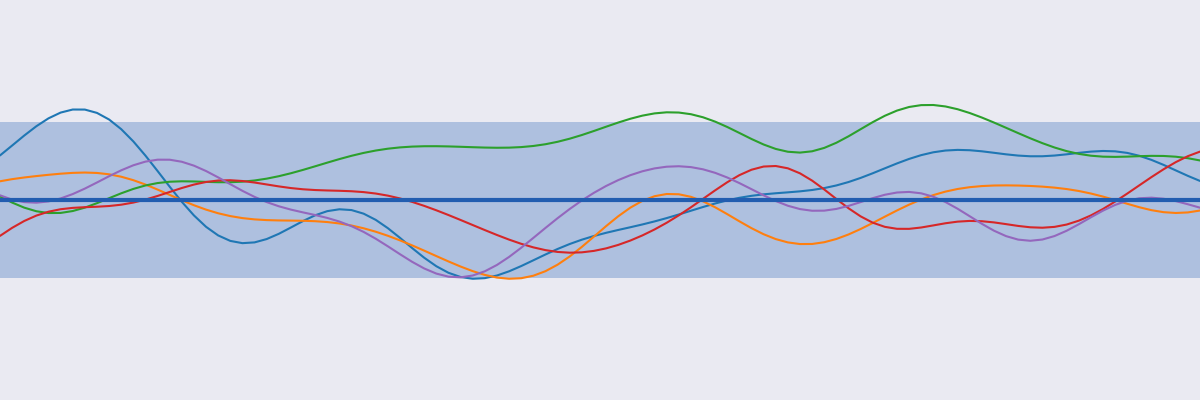
\includegraphics[width=\linewidth]{img_hyperopt/gp_prior.png}
	\caption{Gaussian process prior using a squared exponential kernel. The thin colored lines are samples drawn from the Gaussian process. The thick blue line represents the mean of the distribution and the blue area around is the $95 \%$ prediction interval, i.e. all drawn samples will be in this interval with a probability of $95 \%$ (for a Normal distribution this is equal to $1.96 \sigma$)}
	\label{fig:gp_prior}
\end{figure}

In probabilistic terms, the unfitted Gaussian process corresponds to the prior $p \left( \mathrm{y} \right)$. Given a set of observed points $(\mathrm{X}, \mathrm{y})$ and a set of points we want to predict $(\mathrm{X_*}, \mathrm{y_*})$, the prior corresponds to $p\left( \mathrm{y_*} | \mathrm{X_*}, \theta \right)$ ($\theta$ are the hyper-parameters of the model which we will deal with later). We are interested in the posterior $p\left( \mathrm{y_*} | \mathrm{X_*}, \mathrm{X}, \mathrm{y}, \theta \right)$ i.e. the distribution of the new points conditioned on the points we have already observed. From probability theory we know that the posterior is:

\begin{equation}
    p\left( \mathrm{y_*} | \mathrm{X_*}, \mathrm{X}, \mathrm{y}, \theta \right)
    =
    \frac{p\left( \mathrm{y}, \mathrm{y_*} | \mathrm{X}, \mathrm{X_*}, \theta \right)}{p\left( \mathrm{y} | \mathrm{X}, \theta \right)}
\end{equation}

The numerator is called the joint distribution and the denominator is the marginal likelihood. First, we compute the joint distribution:

\begin{equation}
    \begin{bmatrix}
    \mathrm{y} \\
    \mathrm{y_*}
    \end{bmatrix}
    \sim
    \mathcal{N} \left( 0, 
    \begin{bmatrix}
    K(\mathrm{X}, \mathrm{X}) & K(\mathrm{X}, \mathrm{X_*}) \\
    K(\mathrm{X_*}, \mathrm{X}) & K(\mathrm{X_*}, \mathrm{X_*})
    \end{bmatrix}
    \right)
\end{equation}

Training a Gaussian process simply means pre-computing $K(\mathrm{X}, \mathrm{X})$, i.e. the covariance between the data points. At inference, we compute the covariance $K(\mathrm{X_*}, \mathrm{X_*})$ between the points we want to predict, and the covariance between the points we have observed and the points we want to predict $K(\mathrm{X}, \mathrm{X_*})$. And since the covariance matrix is symmetrical, $K(\mathrm{X_*}, \mathrm{X}) = K(\mathrm{X}, \mathrm{X_*})^T$. For notational simplicity we will denote them $K$, $K_*$ or $K_*^T$ and $K_{**}$.

But the joint distribution is not enough, it will generate functions that do not match the observed data. The posterior is obtained by conditioning the joint distribution to the observations, and because every term involved is a Gaussian distribution, the posterior can be simplified to the following equation:

\begin{equation}
    p\left( \mathrm{y_*} | \mathrm{X_*}, \mathrm{X}, \mathrm{y}, \theta \right)
    =
    \mathcal{N} \left( K_* K^{-1} y, 
    K_{**} - K_* K^{-1} K_*^T \right)
\end{equation}

This is the equation to compute when predicting new points. Most of the cost of the computation is in inverting the covariance matrix. By construction it is always positive semi-definite and is positive definite if its rows and columns are linearly independent. This is always true in the context of Bayesian optimization as long as the points in the training set are unique. Therefore the covariance matrix admits a unique Cholesky decomposition which is faster to compute and invert than directly computing the inverse of the covariance matrix. 

\begin{figure}[htb]
    \centering
    \begin{subfigure}[b]{\textwidth}
        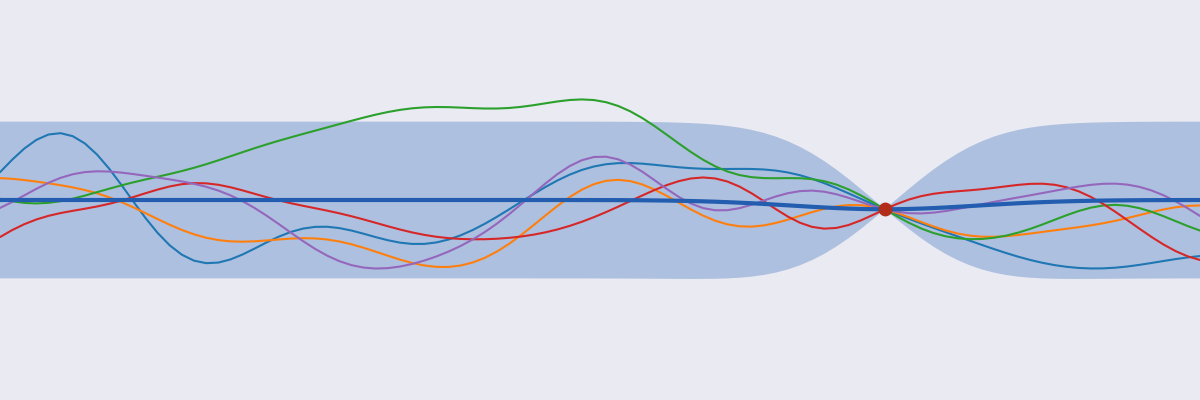
\includegraphics[width=\textwidth]{img_hyperopt/gp_posterior_1_point}
    \end{subfigure}

    \begin{subfigure}[b]{\textwidth}
        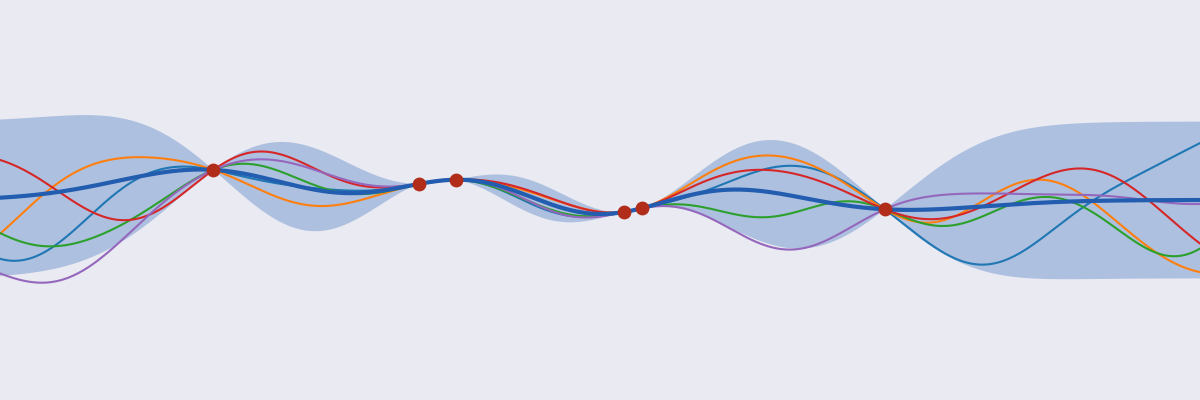
\includegraphics[width=\textwidth]{img_hyperopt/gp_posterior_6_point}
    \end{subfigure}
    \caption{Gaussian process posterior after fitting one point on top, six on the bottom. All the samples pass through those points and the variance is lower close to them.}
    \label{fig:gp_posterior}
\end{figure}

Figure~\ref{fig:gp_posterior} shows how samples from this distribution look like on a one dimensional problem. Each sample must go through every observed point, and the closer the points are, the less freedom the samples have to change. Outside of the range of observed points, the distribution quickly reverts to its prior. This is a property of this kernel, where the influence of a point on the value of another decays exponentially with their relative distance.

So far we have assumed for simplification that the data is noise-free, however it is important to note that Gaussian processes are particularly well-adapted for dealing with noisy data. See~\textcite{rasmussen2005} for the changes to the equations.

We glossed over the choice of kernel until now. The most common is the one we used so far, the squared exponential kernel of Equation~\ref{eq:sqexp}.

This kernel has two hyper-parameters $\theta = \{ \sigma^2 , l \}$. $\sigma^2$ controls the scale of the predicted output and $l$ is a vector of same dimensionality as $\mathrm{x}$ called the characteristic length-scale which measures how much a change along each dimension affects the output. A low value means that a small change in the input results in a big change in the output, as shown in Figure~\ref{fig:gp_lengthscale}.

\begin{figure}[htb]
    \centering
    \begin{subfigure}[b]{\textwidth}
        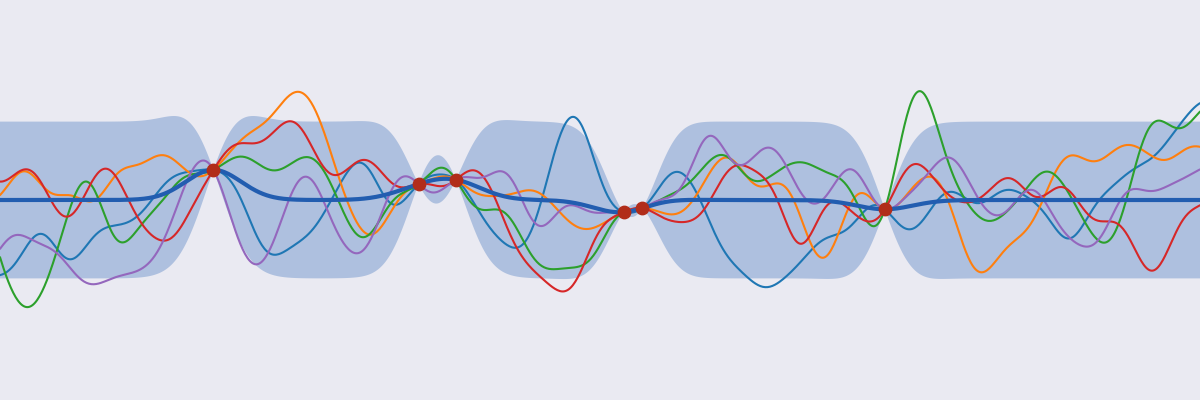
\includegraphics[width=\textwidth]{img_hyperopt/gp_lengthscale_small}
        \caption{$l = 0.3$}
    \end{subfigure}

    \begin{subfigure}[b]{\textwidth}
        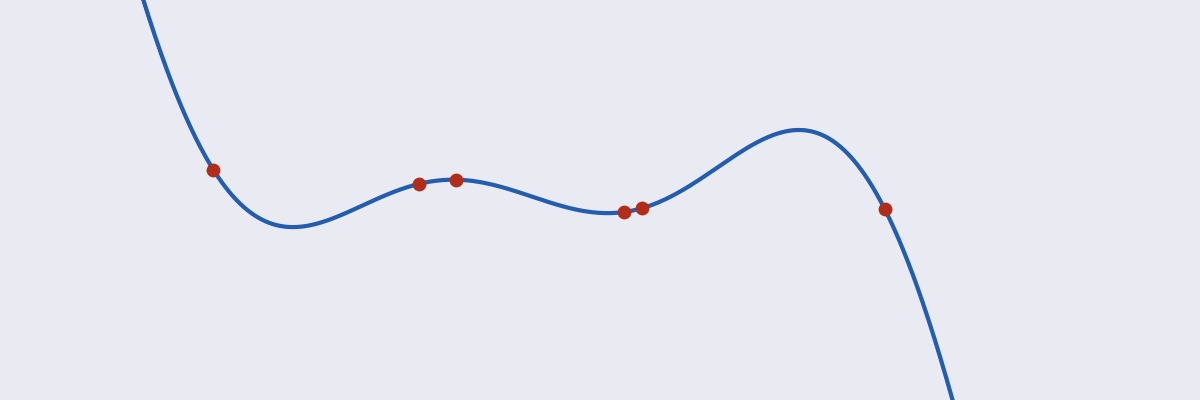
\includegraphics[width=\textwidth]{img_hyperopt/gp_lengthscale_big}
        \caption{$l = 3$}
    \end{subfigure}
    \caption{Gaussian process posterior after six points with different length-scale. On the top with a low length-scale, data points are almost irrelevant, the Gaussian process returns to its prior almost immediately. On the bottom, the GP has a very high confidence in its prediction.}
    \label{fig:gp_lengthscale}
\end{figure}

The samples from this kernel are very smooth, and are in fact infinitely differentiable. This is usually too unrealistic for the process we are modelling. In the context of Bayesian optimization, and noting $r = || \mathrm{x} - \mathrm{x'} ||_2$, a more realistic alternative is the Matérn $5/2$ kernel:
\begin{equation}
    k(r) = \sigma^2 \left( 1 + \frac{\sqrt{5}r}{l} + \frac{5r^2}{3l^2} \right) \exp \left( - \frac{\sqrt{5}r}{l}\right)
\end{equation}

The Matérn covariance functions are a class of kernel with two parameters $l$ and $\nu$. The hyper-parameters $\sigma^2$ and $l$ have the same role as for the squared exponential kernel and $\nu$ is a measure of how smooth the function is. The chosen value of $\nu = 5/2$ means that the samples will be twice differentiable, $\nu = 1/2$ results in a very rough function while $\nu \to \infty$ is the squared exponential kernel. $\nu = 5/2$ is a good compromise between too smooth and too difficult to optimize $\theta$ as many point estimate methods require twice differentiability (\textcite{snoek2012NIPS}). Figure~\ref{fig:gp_matern} shows what samples from these kernels look like.

\begin{figure}[htb]
    \centering
    \begin{subfigure}[b]{\textwidth}
        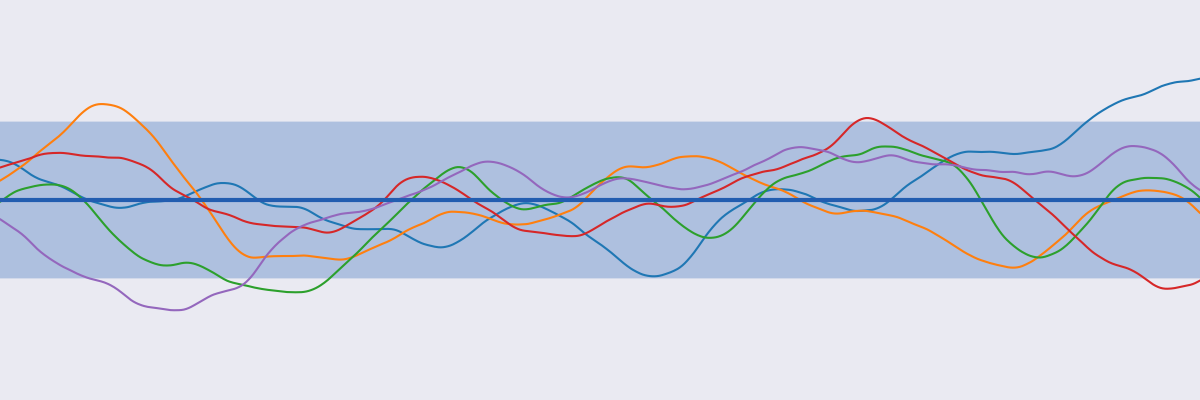
\includegraphics[width=\textwidth]{img_hyperopt/gp_matern_prior}
    \end{subfigure}

    \begin{subfigure}[b]{\textwidth}
        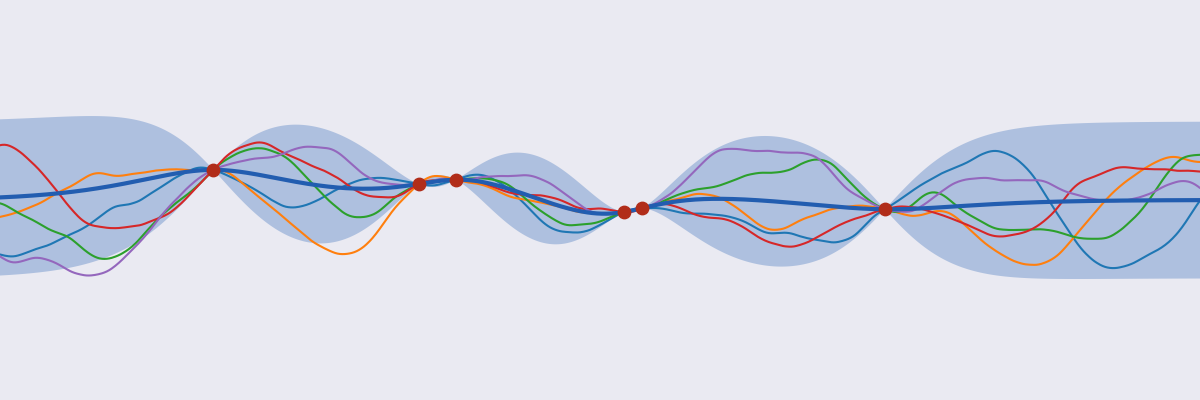
\includegraphics[width=\textwidth]{img_hyperopt/gp_matern_posterior}
    \end{subfigure}
    \caption{Gaussian process using a Matérn $5/2$ kernel. On the top, the prior. On the bottom, the posterior after fitting six points.}
    \label{fig:gp_matern}
\end{figure}

The presented kernels have the common property of being stationary, i.e they depend only of $\mathrm{x} - \mathrm{x'}$. They are invariant to translation. It is particularly relevant in the context of hyper-parameter optimization as the kernels make no difference between values of 3 and 2 or 1000 and 999. Depending on the meaning of the hyper-parameters, this is not desirable. A solution is to use a non-stationary kernel, which we discuss in Section~\ref{ssec:nosta}.

Another problem of those kernels is that they have themselves hyper-parameters $\theta$ which need to be chosen. As said before, $l$ is the characteristic length-scale. By construction of those covariance functions, and as shown by~\textcite{neal1996phd}, the inverse of the length-scale determines how relevant an input is. In the context of hyper-parameter optimization, it can help to choose which hyper-parameters to tune carefully. It is therefore very important to select the correct value for $l$. 

There are two ways to learn $\theta$. The first way is to maximize the marginal likelihood, which can be derived as:  
\begin{equation}
	\log p\left(\mathrm{y} | \mathrm{X}, \theta \right) = - \frac{1}{2} \mathrm{y}^T K^{-1} \mathrm{y} - \frac{1}{2} \log |K| - \frac{n}{2} \log 2 \pi
\end{equation}

The optimization can be done with any off-the-shelf method, eventually with multiple restarts as there are no guarantee of a unique optimum. 
%For example, the scikit-learn (\textcite{pedregosa2011sklearn}) implementation uses BFGS with 10 restarts by default.

The other solution is to not learn $\theta$ at all and instead marginalize the hyper-parameters, i.e. at the inference step compute:
\begin{equation}
    p\left( \mathrm{y_*} | \mathrm{X_*}, \mathrm{X}, \mathrm{y} \right)
    = \int p\left( \mathrm{y_*} | \mathrm{X_*}, \mathrm{X}, \mathrm{y}, \theta \right) p \left( \theta | \mathrm{X}, \mathrm{y} \right) d\theta
\end{equation}

This integral is usually intractable but can be approximated by sampling methods. \textcite{murray2010NIPS} use slice sampling, \textcite{garbuno2016CSDA} use asymptotically independent Markov sampling and \textcite{titsias2011} review different Monte Carlo methods used for this problem.

For a more extensive description of Gaussian Processes, see~\textcite{rasmussen2005}.

%%%%%%%%%%%%%%%%%%%%%%%%%%%%%%%%%%
\subsection{Acquisition Functions}
\label{ssec:acqfunc}

TODO:
\begin{itemize}
    \item Figure PI vs EI
    \item Should I talk about other functions, even if we didn't use them ? (Upper Confidence Bound, Thompson Sampling, Entropy-search Portfolio)
\end{itemize}

In the context of Bayesian optimization, the Gaussian process gives for each set of hyper-parameters an estimation of the performance of the corresponding model and the uncertainty of the Gaussian process in its estimation. But we do not have a way to decide which model is the most interesting to train. Do we pick a model that will be slightly better than our best current model, i.e. where the Gaussian process gives low uncertainty, or do we pick a model with high uncertainty but which could have terrible performance ? There is an exploration/exploitation trade-off. It is the role of the acquisition function to determine which model to train.

One acquisition function is the Probability of Improvement (\textcite{kushner1964}). It chooses the model which has the highest probability of having better results than a target, which is usually picked to be the loss of the current best model. The \textit{PI} is defined as below, where $\Phi$ is the Normal cumulative distribution function, $\mathrm{x}$ represents a given set of hyper-parameters, $y_*$ is the minimum loss found so far, $\mu$ is the mean returned by the Gaussian process and $\sigma$ the variance:
\begin{equation}
    PI(\mathrm{x}) = \Phi \left( \frac{y_* - \mu(\mathrm{x})}{\sigma(\mathrm{x})}\right)
\end{equation}

The problem with this function is that it is highly sensitive to the choice of target. The simplest is to choose the minimum loss found so far, but the \textit{PI} will then sample models very close to the corresponding model completely foregoing exploration. A better target is how much to improve on the minimum loss. But that's very inconvenient because we usually have no idea how much better we can get. Should we try to find a model $1 \%$ better ? $5 \%$ ? $25 \%$ And if we pick too big of an improvement, the function will simply select the models with the highest uncertainty.

Instead, we can use the Expected Improvement function (\textcite{schonlau1998}) which build on the Probability of Improvement as below where $\phi$ is the normal density function.:
\begin{equation}
	EI(\mathrm{x})  = \sigma (\mathrm{x}) [u\Phi(u)+\phi(u)]
\end{equation}
with
\begin{equation}
	u = \frac{y_* - \mu(\mathrm{x})}{\sigma(\mathrm{x})}
\end{equation}

\textit{EI} is obtained by taking the expectation of the improvement function (\textcite{shahriari2016IEEE}), defined as:
\begin{equation}
	I(\mathrm{x}) = \left(y_* - \mu(\mathrm{x}) \right) \mathds{1} \left(y_* > \mu(\mathrm{x}) \right)
\end{equation}

This function is equal to $0$ if the predicted mean is less than the best loss found so far (which means that there is no improvement), otherwise it is proportional to the gap between the predicted mean and best loss. 

The Expected Improvement has one big advantage over the Probability of Improvement. The target is always the minimum loss found so far, meaning that there is no need to guess a threshold of improvement. 

An extended discussion on the trade-offs between Probability of Improvement and Expected Improvement can be found in~\textcite{jones2001}.

%%%%%%%%%%%%%%%%%%%%%%%%%%%%%%%%%%
\subsection{Bayesian Optimization}

TODO:
\begin{itemize}
    \item Figure step-by-step BO
\end{itemize}

Let us resume the situation. We want to find the best model in a large family of models in a reasonable amount of time. We have already trained some models and are trying to decide which model to train next. First, we fit a Gaussian process on the models already trained, with the hyper-parameters as the input, and the loss of the corresponding model as the output. We then sample new combinations and have them predicted by the Gaussian process. For each sample, we also compute the Expected Improvement. The next model to train is the one with the highest \textit{EI}. Once it is trained, we fit again the Gaussian process with the new information, and we repeat the process until we run out of time or we obtain a model good enough for our purposes. Figure~\ref{fig:bo} shows this process on a one-dimensional problem.

\begin{figure}[htb]
	\centering
	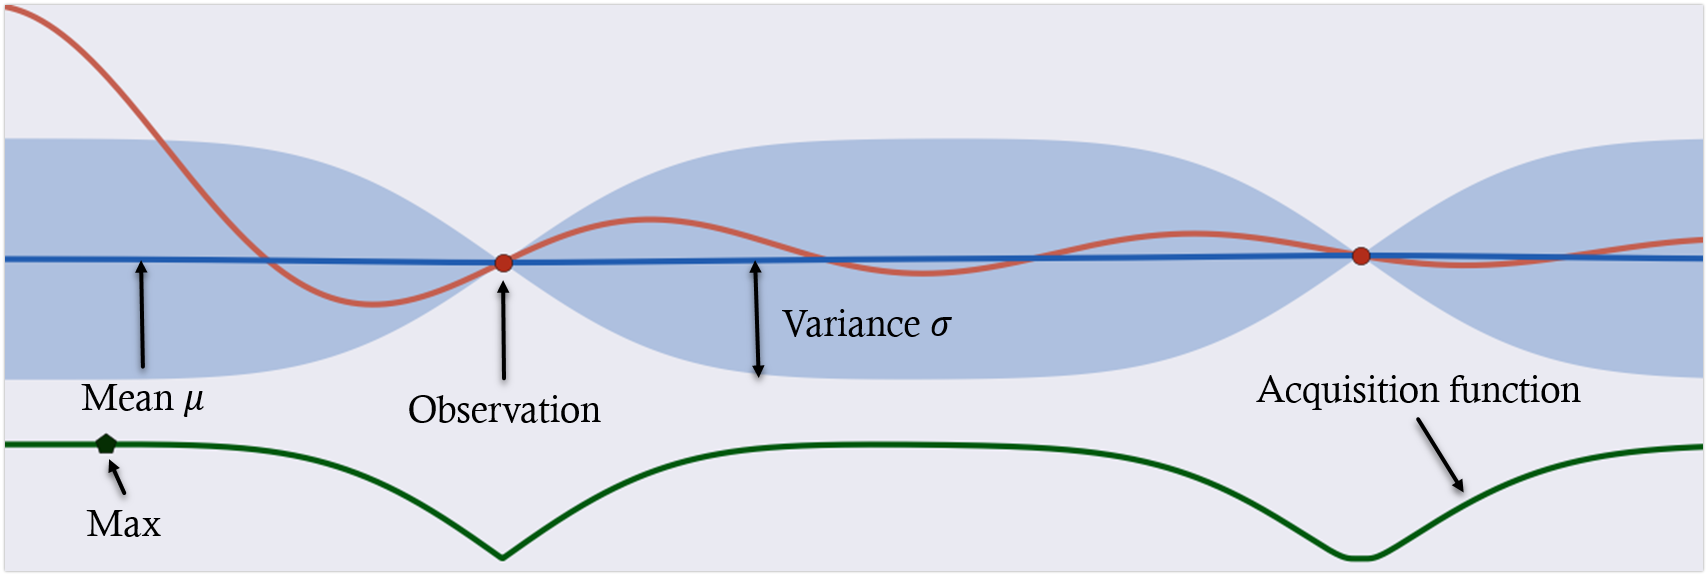
\includegraphics[width=\linewidth]{img_hyperopt/bo.png}
	\caption{Bayesian Optimization on a one dimensional function. The orange curve is the true loss function, the blue one is the prediction of the Gaussian process. The green curve is the acquisition function. The next evaluation will be at the maximum of the green curve.}
	\label{fig:bo}
\end{figure}

Some questions remain. How to pick the first model ? Select a random configuration of hyper-parameters from the hyper-parameter space. Should the Gaussian process predict the loss on the training set or on the validation set ? The loss on the validation set is to be preferred. How to sample configurations ? Uniformly from the hyper-parameter space. How many configurations should be sampled before selecting a model to train ? As many as reasonably possible. The step of selecting a model should be much faster than training it, and most of the cost of Bayesian optimization should be in the inversion of the Gram matrix (see Section~\ref{ssec:practical} for details).

%Hyperopt~\textcite{bergstra2013ICML}

%Practical~\textcite{snoek2012NIPS}

%%%%%%%%%%%%%%%%%%%%%%%%%%%%%%%%%%
\subsection{Practical Challenges}
\label{ssec:practical}

%==One important aspect of this method is that the training time of the model is a dimension of the hyper-parameter space. This means that the method is free to choose how long to train each model. In practice we found that it prefers longer training time, even though it looks like a lower training time is enough to get a good estimate of the worth of the model and would allow the evaluation of more models. This is a flaw of the method, which lacks an explicit notion of budget and a way to best exploit it.

\subsubsection{Conditional spaces}

TODO
\begin{itemize}
    \item Describe cylindrical embeddings
    \item Describe tree of Parzen estimator
\end{itemize}

The version of Bayesian optimization we presented deals efficiently with both discrete and continuous hyper-parameters. But what about conditional hyper-parameters ? For example, some hyper-parameters could be specific to a particular layer and one hyper-parameter could control the number of layers. But then, what happens to the hyper-parameters of a non-existent layer ? With a Gaussian process, we need to give them a value and it means there will be many configurations that corresponds to the same model. In practice, we can ignore those cases, and the Gaussian process will eventually give a low uncertainty in those regions and pick models elsewhere. But this is extremely wasteful as we will retrain the same model many times before this happens ! 

One solution is to use a specialized kernel called a cylindrical kernel (\textcite{swersky2013},~\textcite{oh2018}).

Another solution is to not use a Gaussian process at all. It has been our model of choice so far but other alternatives exist. One such alternative is tree-structured Parzen estimator (\textcite{bergstra2011NIPS}).

\subsubsection{Parallelization}

Open problem using GP

See combination with Hyperband for a potential solution

\subsubsection{Non-stationarity}
\label{ssec:nosta}

Input Warping~\textcite{snoek2014ICML}

\subsubsection{Scaling}

Doesn't work well in high-dimension or with thousands of data points

Conditional neural processes ?

%%%%%%%%%%%%%%%%%%%%%%%%%%%%%%%%%%
\subsection{Contribution: Incremental Cholesky decomposition}

TODO:
\begin{itemize}
    \item Rewrite the explanation
    \item Should I put the full proof of the results here ? In an appendix ?  
\end{itemize}

One of the big timesink of GP: computing the Cholesky decomposition. But in BO, the Gram matrix between calls is mostly the same, just with new rows. So we can store the decomposition and just update it.

==An important property of Gaussian processes is that the Gram matrix $K$ always has a unique Cholesky decomposition ($K$ is definite positive). This property is used in practice for the prediction of the mean and variance because it is necessary to invert $K$, and it is much more efficient to invert the Cholesky decomposition $L$.

==We use here the structure of the Gram matrix and a property of Bayesian optimization in order to reduce significantly the cost of the decomposition. The property is the following: at every call of the Gaussian process, our training set contains $n$ points from before and $k$ new points. By keeping the order of the points, the new Gram matrix is always structured as follows:
\begin{equation}
	K_{(n+k,n+k)} = 
    \begin{pmatrix}
    K_{(n,n)} & K_{(k,n)}^T \\
    K_{(k,n)} & K_{(k,k)}
  \end{pmatrix}
\end{equation}

==Moreover,
\begin{equation}
	 K_{(n,n)} = L_{(n)} L_{(n)}^T
\end{equation}
is already known. The question is then: can we compute $L_{(n+k)}$ from $L_{(n)}$ and the $k$ new points? The answer is positive, and after a bit of arithmetics omitted here, we get this:
\begin{equation}
  L_{(n+k)} = 
  \begin{pmatrix}
    L_{(n)} & 0 \\
    K_{(k,n)} (L_{(n)}^T)^{-1} & L_{(k)}
  \end{pmatrix}
\end{equation}

==It is also possible to get a formula for $ L_{(n+k)}^{-1}$:
\begin{equation}
  L_{(n+k)}^{-1} =
  \begin{pmatrix}
    L_{(n)}^{-1} & 0 \\
    - L_{(k)}^{-1} K_{(k,n)} (L_{(n)}^T)^{-1} L_{(n)}^{-1} & L_{(k)}^{-1}
  \end{pmatrix}
\end{equation}

==The complexity of the Cholesky decomposition is $O\left(\frac{(n+k)^3}{3}\right)$. In our case, this becomes $O\left(\frac{k^3}{3}\right)$ since it is still necessary to compute the decomposition of the $k$ new points.

%%%%%%%%%%%%%%%%%%%%%%%%%%%%%%%%%%%%%%%%%%%%%%%%%%%%%%%%%%%%%%%%%%%%%%%%%%%%%%%%%%%%%%%%%%%%%%%
\section{Contribution: Combining Bayesian Optimization and Hyperband}
\label{sec:cap}

This section describes and extend work that was presented at CAp 2017 (\textcite{bertrand2017CAp}).

%%%%%%%%%%%%%%%%%%%%%%%%%%%%%%%%%%
\subsection{Hyperband}
\label{ssec:hyperband}

A property of neural networks is that their training is iterative, usually some variant of gradient descent. A consequence is that it is possible to interrupt training at any time, evaluate the network, then resume training. This is the property Hyperband (\textcite{li2017ICLR}) takes advantage of.

The principle is simple: pick randomly a group of configurations from a uniform distribution, train the corresponding networks partially, evaluate them, resume training of the most performing ones, and so on until a handful of them have been trained to completion. Then pick a new group and repeat the cycle until exhaustion of the available resources.

But a problem appears: at which point in the training can we start evaluating the models? Too soon and they will not have started to converge, making the evaluation meaningless, too late and we have wasted precious resources training under-performing models. Moreover, we do not know how to find that point and it changes between tasks. Hyperband's answer is to divide a cycle into brackets. Each bracket has the same quantity of resource at its disposal. The difference between brackets is the point at which they start evaluating the models. The first bracket will start evaluating and discarding models very early, allowing it to test a bigger number of configurations, while the last bracket will test only a small number of configurations but will train them until the end.

The algorithm is controlled by two hyper-parameters: the maximal quantity of resources $R$ that can be allocated to a given model, and the proportion of configurations $\eta$ kept at each evaluation. We chose $R = 27$ minutes and $\eta = 3$, which means that we keep $1/3$ of models at each evaluation.

%%%%%%%%%%%%%%%%%%%%%%%%%%%%%%%%%%
\subsection{Combining the methods}

%%%%%%%%%%%%%%%%%%%%%%%%%%%%%%%%%%
\subsection{Random Search Efficiency}
\label{ssec:random}

TODO:
\begin{itemize}
    \item Find where to put this section
\end{itemize}

How many models of a hyper-parameters space should be trained in order to be reasonably certain to have trained one of the best ? If we knew the loss $l_{min}$ of the best model, how long would it take to find a model with a loss such as $l \leq (1 + \alpha) l_{min}$ ?

Let $N$ be the total number of models in the hyper-parameters space, $M$ the number of models satisfying our performance criteria (alternatively, the $M$ best models of the space) and $n$ the number of models to train.

Considering random search chooses models uniformly, the probability of drawing one of the best model the first time is simply $\frac{M}{N}$. The second time, it is $\frac{M}{N - 1}$ since we do not allow redrawing a model. We can therefore define the probability of not drawing any satisfying models after $n$ draw as:

\begin{equation}
    P \left( Y = n \right) = \prod_{k = 0}^{n} \left( 1 -  \frac{M}{N - k} \right)
\end{equation}

where $Y$ is the random variable of failing to draw an acceptable models $n$ draw in a row. This is a particular case of the hypergeometric distribution. From there, the probability of drawing an acceptable model at the $n$-th draw is:

\begin{equation}
    P\left(X = n \right) = \frac{M}{N - n} \prod_{k = 0}^{n - 1} \left( 1 -  \frac{M}{N - k} \right)
\end{equation}

$X$ is the random variable of drawing an acceptable model after $n - 1$ bad draws. The probability of drawing an acceptable model in the first $n$ draws is:

\begin{equation}
    P\left(X \leq n \right) = \sum_{k = 0}^{n} P\left(X = k \right)
\end{equation}



%%%%%%%%%%%%%%%%%%%%%%%%%%%%%%%%%%
\subsection{Experiments on CIFAR-10}

TODO:
\begin{itemize}
    \item Results on hyperband
    \item Results on hyperband + bo
\end{itemize}

\subsubsection{Setup}

In order to compare the performance of the different hyper-parameter optimization methods, we devised a hyper-parameter space containing 600 models and trained them all on the CIFAR-10 dataset (\textcite{krizhevsky2009}).

The dataset is composed of 60 000 images equally divided in 10 classes. The images are 32x32 RGB images. The training set contains 50 000 images, the test set 10 000.

Since the goal of the experiment is not to beat the state-of-the-art on the dataset, the selected hyper-parameter space and the resulting models are small and simple. Each model is trained for a total of 10 minutes. 

We then compare in which order the different methods selected the models. The methods are evaluated on how long it took them to select the best model, but also on the average performance of the models selected, i.e. if we rank the models by their performance, how close were each method from selecting the models in that order.

However one run is not enough to conclude that Bayesian optimization on average is more efficient than random search. Due to the huge computing cost, we cannot do hundreds of runs with different seed and retrain each network every time. But if we do not retrain the network but change the seeds of the search policy, we can simulate hundreds of runs at a low cost. 

There are a total of $600!$ way to explore this space, but because we do not retrain the models, all the randomness in Bayesian optimization is in the choice of the first model, leaving us with only 600 possible paths through this space. We computed them all, then randomly selected 600 ordering for random search.

\subsubsection{Models distribution}

\begin{figure}[htb]
	\centering
	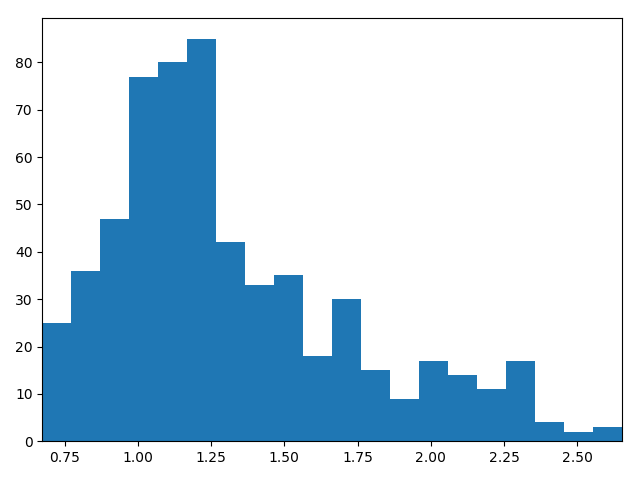
\includegraphics[width=0.7\linewidth]{img_hyperopt/cifar_hist.png}
	\caption{Distribution of the models performance.}
	\label{fig:cifar_hist}
\end{figure}

Before comparing the search methods, we look at the distribution of models performance in Figure~\ref{fig:cifar_hist}. A few models are really good, most are average and then there is a long trail of progressively worse models. It looks like a skew normal distribution. 

We of course can't extrapolate that every hyper-parameter space will have a distribution like this, but we assume for now that this is the case for hyper-parameter spaces designed in practice.

Since the distribution is not uniform, there is a difference between models in the top $5 \%$ of models and models that have a performance within $5 \%$ of the performance of the best model. In this case, there are 30 models in the top $5 \%$ of models (since there are 600 models), but only 6 are within $5 \%$ of the performance of the best model. In this case, the 30-th best model is within $18 \%$ of the best model.

This distinction is important because it changes our evaluation of the methods. We are not simply interested in the average time to find a model in the top x $\%$ of models, but also in the average time to find a model within x $\%$ of the best model.

\subsubsection{Results}

\begin{figure}[htbp]
	\begin{subfigure}[b]{\textwidth}
            \centering
            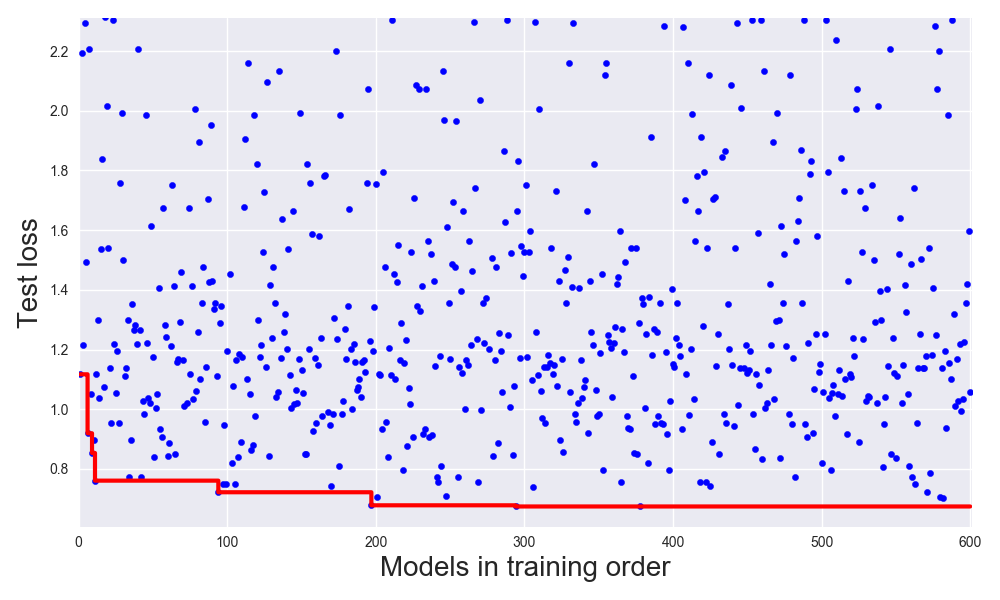
\includegraphics[width=\linewidth]{img_hyperopt/cifar_random}
    \end{subfigure}%
    
    \begin{subfigure}[b]{\textwidth}
            \centering
            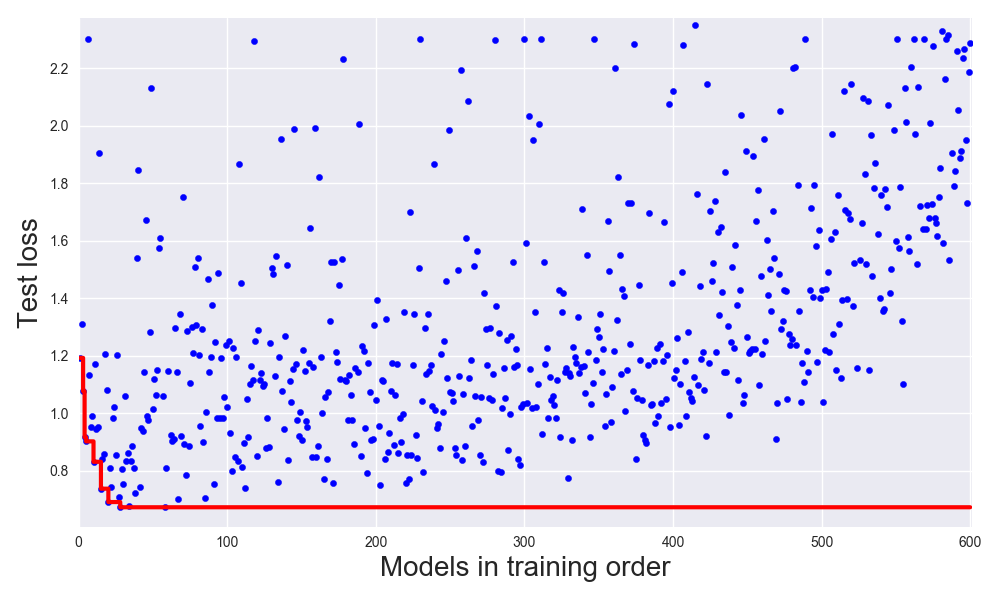
\includegraphics[width=\linewidth]{img_hyperopt/cifar_bo}
    \end{subfigure}%
    \caption{Comparing the model order chosen by random search (top) vs Bayesian optimization (bottom).}
	\label{fig:cifar_loss}
\end{figure}

First, we look at the order in which models where selected during one run, shown in Figure~\ref{fig:cifar_loss}. The blue points represent the test loss of the models in the order the methods selected them, and the red line shows the minimum loss found at a given time. There is a clear trend present for Bayesian optimization where the combinations evaluated later have low performance, suggesting it did learn to predict correctly the performance of untested combination. In this run, it was also able to find the best model much earlier than random search. Random search looks as expected, models performance is uniformly distributed.

\begin{table}[htb]
	\centering
	\begin{tabular}{ | l | c | c | }
		\hline
		 & Random Search & Bayesian optimization \\ 
		\hline
		Best model & $297 \pm 171$ &  \\
		\hline
		Within $1 \%$ & $146 \pm 114$ & \\
		Within $5 \%$ & $87 \pm 75$ & \\
		Within $10 \%$ & $54 \pm 52$ & \\
		\hline
		Top $1 \%$ & $87 \pm 75$ &  \\
		Top $5 \%$ & $18 \pm 17$ &  \\
		Top $10 \%$ & $10 \pm 10$ &  \\
		\hline
	\end{tabular}
	\caption{Average number of draws taken by each method to reach different goals}
	\label{table:search_average}
\end{table}

To confirm these trends, we look at the average number of draws taken by each method to reach different goals (Table~\ref{table:search_average}).

Random search took on average 297 draws before finding the best model, which is within expected range of the theoretical value of 300 draws. If we rank the model by their performance, it took random search an average of 18 draws to find a model in the top $5\%$ and 87 to find a model in the top $1\%$.

[TODO add BO]

\begin{figure}[htb]
	\centering
	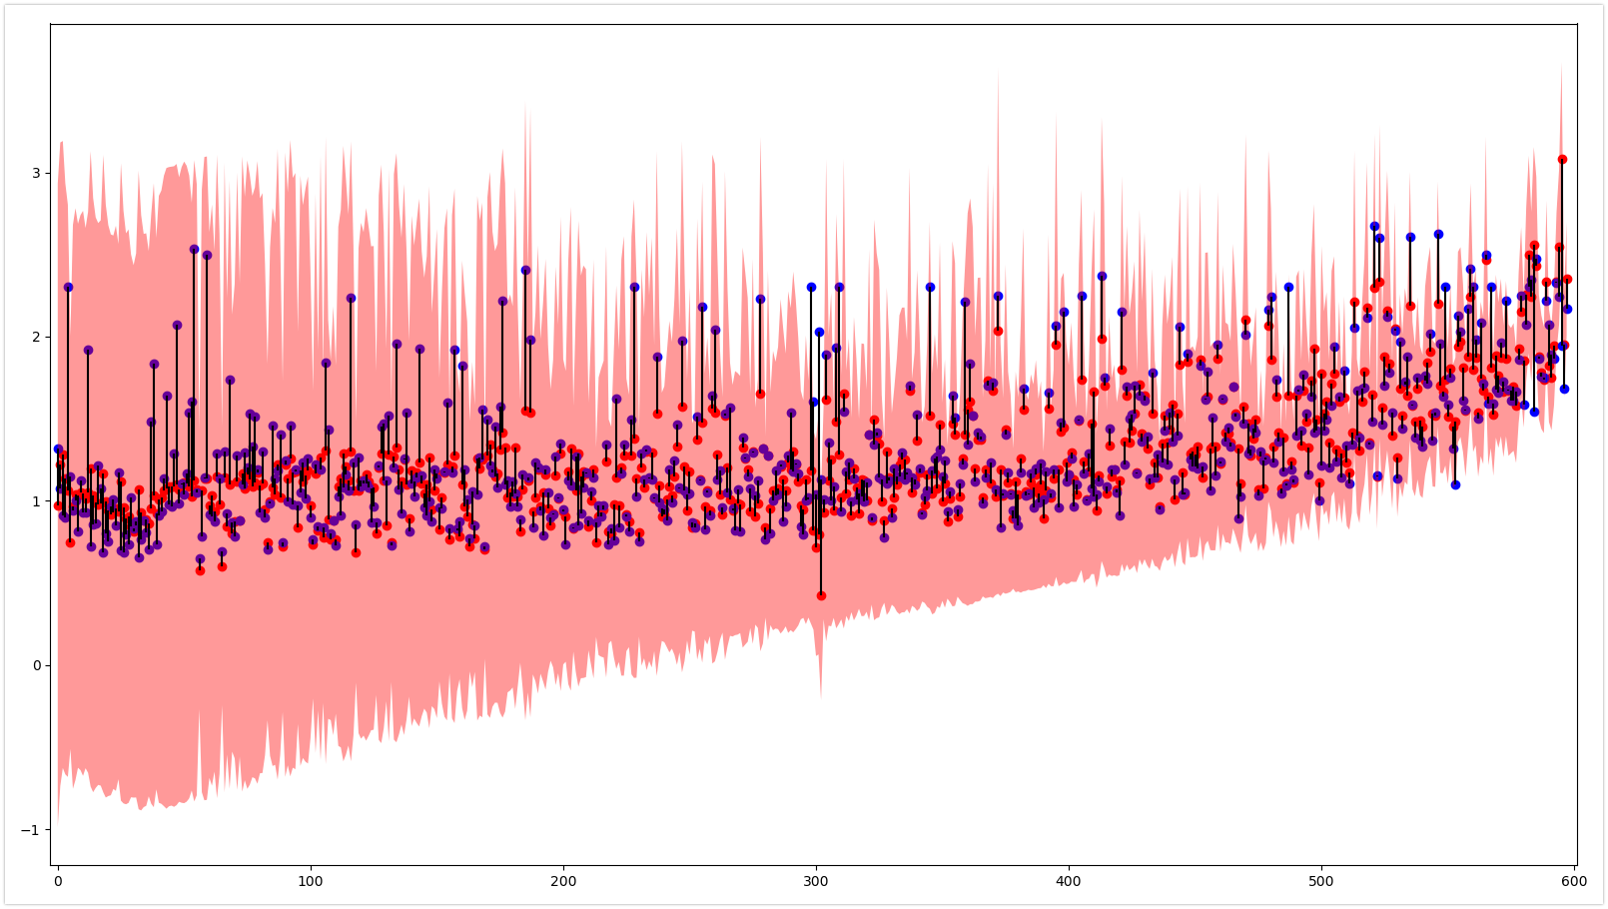
\includegraphics[width=\linewidth]{img_hyperopt/bo_error_time.png}
	\label{fig:bo_error_time}
\end{figure}

%%%%%%%%%%%%%%%%%%%%%%%%%%%%%%%%%%%%%%%%%%%%%%%%%%%%%%%%%%%%%%%%%%%%%%%%%%%%%%%%%%%%%%%%%%%%%%%
\section{Application: Classification of MRI Field-of-View}

This section describes and extends work presented at ISBI 2017 (\textcite{bertrand2017ISBI}).

%%%%%%%%%%%%%%%%%%%%%%%%%%%%%%%%%%
\subsection{Dataset and Problem Description}

\begin{figure}[htb]
        \begin{subfigure}[b]{0.25\textwidth}
                \centering
                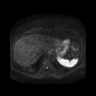
\includegraphics[width=.95\linewidth]{img_hyperopt/Abdomen_785}
        \end{subfigure}%
        \begin{subfigure}[b]{0.25\textwidth}
                \centering
                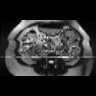
\includegraphics[width=.95\linewidth]{img_hyperopt/Abdomen_1050}
        \end{subfigure}%
        \begin{subfigure}[b]{0.25\textwidth}
                \centering
                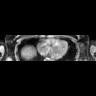
\includegraphics[width=.95\linewidth]{img_hyperopt/Abdomen_5115}
        \end{subfigure}%
        \begin{subfigure}[b]{0.25\textwidth}
                \centering
                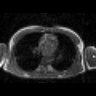
\includegraphics[width=.95\linewidth]{img_hyperopt/Chest_6810}
        \end{subfigure}
        
        \vspace*{2mm}
        
        \begin{subfigure}[b]{0.25\textwidth}
                \centering
                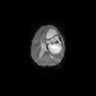
\includegraphics[width=.95\linewidth]{img_hyperopt/Head_13330}
        \end{subfigure}%
        \begin{subfigure}[b]{0.25\textwidth}
                \centering
                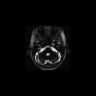
\includegraphics[width=.95\linewidth]{img_hyperopt/Head_14031}
        \end{subfigure}%
        \begin{subfigure}[b]{0.25\textwidth}
                \centering
                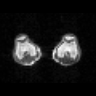
\includegraphics[width=.95\linewidth]{img_hyperopt/Legs_13170}
        \end{subfigure}%
        \begin{subfigure}[b]{0.25\textwidth}
                \centering
                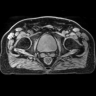
\includegraphics[width=.95\linewidth]{img_hyperopt/Pelvis_23016}
        \end{subfigure}
        \caption{Images from the MR dataset showing the variety of classes and protocols.}
        \label{fig:dataset}
\end{figure}

Given an MRI volume we would like to know which anatomical regions are contained in it and their position in the volume. Since MRI data are acquired in a slice by slice approach, we reduce the problem to a two dimensional classification task of axial slices (into head, chest, abdomen, pelvis, legs and spine).

\begin{table}[htb]
	\centering
	\begin{tabular}{ | l | c | r | }
		\hline
		Body Part & \# Volumes & \# Slices \\ \hline
		Head & 404 & 17011 \\
		Chest & 186 & 6897 \\
		Abdomen & 367 & 15486 \\
		Pelvis & 351 & 17962 \\
		Legs & 99 & 12868 \\
		Spine & 390 & 9790 \\
		\hline
	\end{tabular}
	\caption{Content of the dataset.}
	\label{table:dataset}
\end{table}

The dataset consists of MRI images coming from a variety of hospitals and machines across the world (such as the \textit{Centre Hospitalier Lyon-Sud, France} or \textit{ Johns Hopkins University, USA}). As a consequence the images are highly varied in terms of protocols (see Figure~\ref{fig:dataset}) as well as resolution, number of volumes per class and number of slices per volume. Table~\ref{table:dataset} sums up the content of our dataset.

The dataset is splitted into a training set for the optimization of the weights of the networks, a validation set for model selection (optimization of the hyper-parameters) and a test set for model evaluation (respectively $50 \%$, $25 \%$, $25 \%$ of the database). The separation is done volume-wise to take into account intra-subject slices correlations. Volumes containing multiple classes are split by anatomical regions and can end up in different sets. This raises the difficulty of the task since, in case of overfitting, predictions will be wrong at validation or testing phases.

%We also stratified classes across sets, giving us a proportion of slices per class close to the proportion of volumes per class.

Finally, each slice is subject to a unique step of preprocessing: it is resized to $128 \times 128$ pixels, a good trade-off between time constraints and quality of information.

Data augmentation is used and consists in generating 80 000 images per epoch. The augmentation is done by applying translations, shearing and rotations, zooming, and adding Gaussian noise.

%%%%%%%%%%%%%%%%%%%%%%%%%%%%%%%%%%
\subsection{Baseline Results}

\begin{figure}[htb]
	\centering
	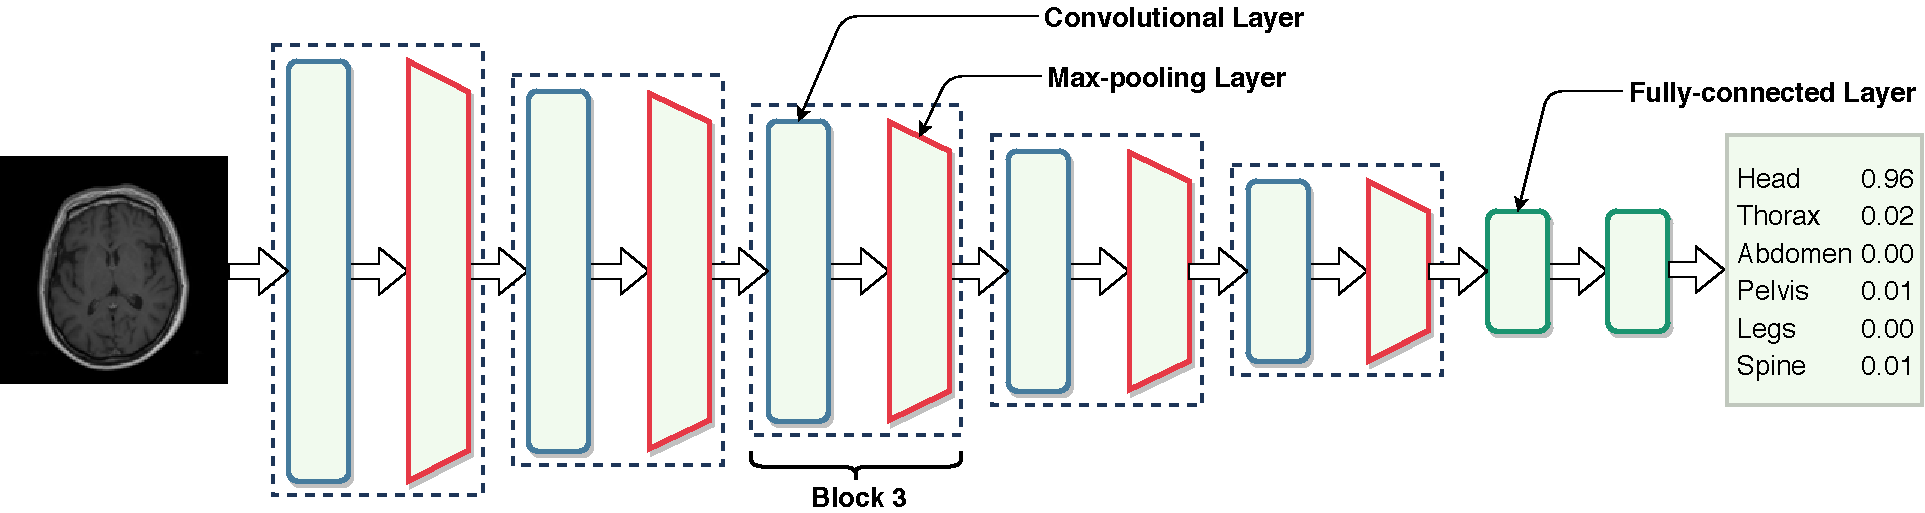
\includegraphics[width=\linewidth]{img_hyperopt/baseline.pdf}
	\caption{Baseline network used to solve the problem.}
	\label{fig:baseline}
\end{figure}

Starting from a standard VGG architecture (\textcite{simonyan2014}), we modified it manually until settling on the following model, shown in Figure~\ref{fig:baseline}: it is divided into 5 blocks, each comprising a convolution layer of 64 filters of size $3\times 3$, followed by a rectified linear unit (ReLu) and a max-pooling layer. The network ends with 2 fully-connected layers (respectively 4096 and 1024 units) interleaved with ReLU activations and terminated with a softmax decision layer. This network was trained by minimizing the categorical cross-entropy loss weighted by class frequency, using stochastic gradient descent (SGD) with a learning rate of $10^{-3}$, Nesterov momentum ($m = 0.9$) and decay ($d = 10^{-6}$) for 30 epochs.

\begin{table}
    \centering
    \newcommand\items{6}   %Number of classes
    \arrayrulecolor{white} %Table line colors
    \noindent\begin{tabular}{cc*{\items}{|E}|}
    \multicolumn{1}{c}{} &\multicolumn{1}{c}{} &\multicolumn{\items}{c}{\textbf{Predicted}} \\ \hhline{~*\items{|-}|}
    \multicolumn{1}{c}{} & 
    \multicolumn{1}{c}{} & 
    \multicolumn{1}{c}{\rot{Head}} & 
    \multicolumn{1}{c}{\rot{Chest}} & 
    \multicolumn{1}{c}{\rot{Abdomen}} &
    \multicolumn{1}{c}{\rot{Pelvis}} & 
    \multicolumn{1}{c}{\rot{Legs}} & 
    \multicolumn{1}{c}{\rot{Spine}} \\ \hhline{~*\items{|-}|}
    \multirow{\items}{*}{\rotatebox{90}{\textbf{Actual}}} 
    &Head  & 96 & 0 & 1 & 2 & 1 & 0   \\ \hhline{~*\items{|-}|}
    &Chest  & 1 & 57 & 13 & 28 & 1 & 0   \\ \hhline{~*\items{|-}|}
    &Abdomen  & 0 & 1 & 88 & 10 & 0 & 1   \\ \hhline{~*\items{|-}|}
    &Pelvis  & 1 & 0 & 9 & 81 & 8 & 1   \\ \hhline{~*\items{|-}|}
    &Legs  & 0 & 0 & 0 & 19 & 81 & 0   \\ \hhline{~*\items{|-}|}
    &Spine  & 0 & 1 & 3 & 2 & 0 & 94   \\ \hhline{~*\items{|-}|}
    \end{tabular}
    \caption{Confusion matrix for the baseline on the test set, in percent.}
	\label{table:conf_matrix_baseline}
\end{table}

We achieve a $14 \%$ error rate with most of the error focused on the chest. Examining the confusion matrix (Table~\ref{table:conf_matrix_baseline}), we note that the abdomen, pelvis and legs images have most of their errors located with anatomically adjacent regions. Further examinations of the misclassified images revealed they were for the most part located at the boundaries of their classes. These errors make sense as these boundaries are ill-defined and varies from one volume to the next. 

%%%%%%%%%%%%%%%%%%%%%%%%%%%%%%%%%%
\subsection{Hyper-parameter Optimization}

TODO:
\begin{itemize}
    \item Redo results
    \item Best networks figure ?
    \item Confusion matrix baseline vs best vs ensemble
\end{itemize}

\begin{figure}[htb]
	\centering
	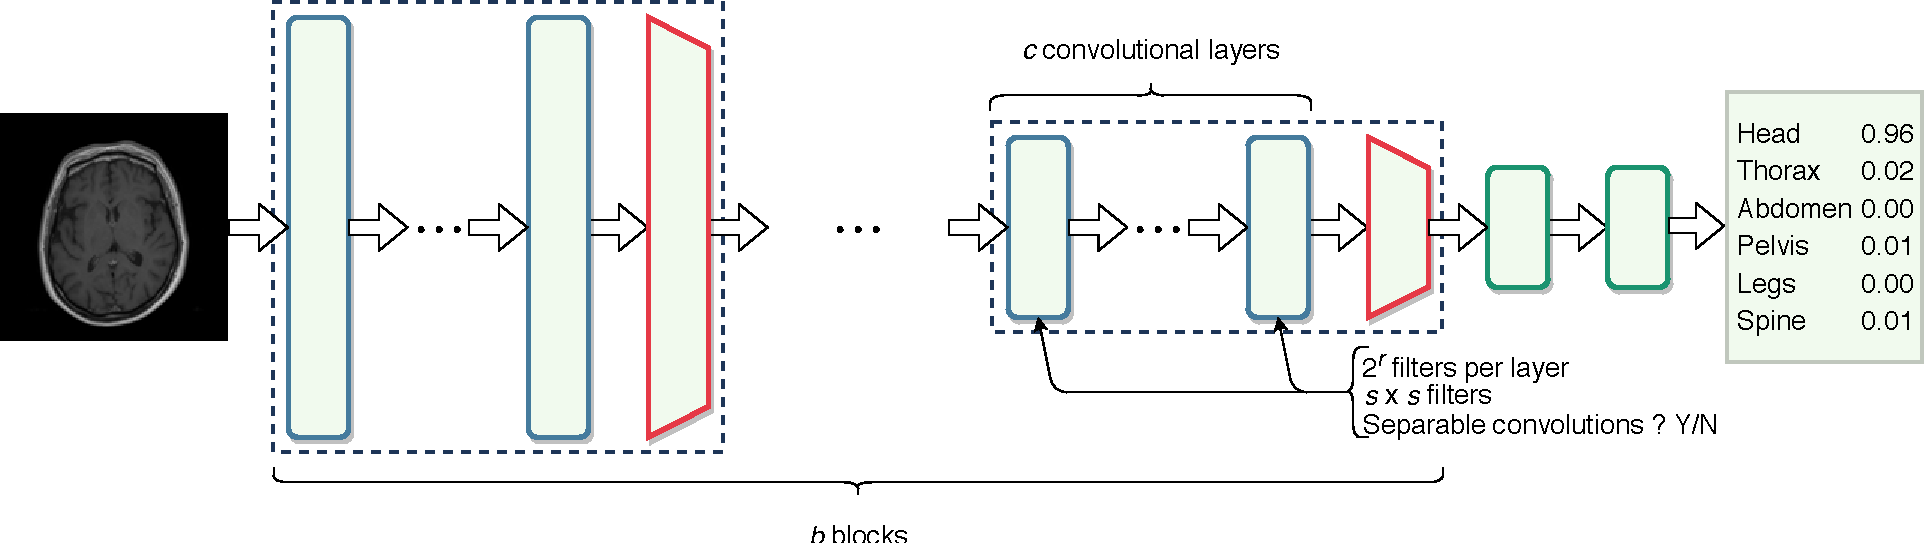
\includegraphics[width=\linewidth]{img_hyperopt/hyperspace.pdf}
	\caption{Variations on the baseline allowed in our search.}
	\label{fig:hyperspace}
\end{figure}

By relaxing some structural parts of our baseline architecture we define a large family of models. This hyper-parametric family has the following structure (see Figure~\ref{fig:hyperspace}): (1) $b$ convolution blocks, each including $c$ convolutional layers of $2^r$ filters of size $s \times s$ interleaved with ReLU activations and terminated by a max-pooling layer, (2) the fully-connected layers as in our baseline architecture, and (3) a final softmax decision layer. Moreover, the convolutions can be separable or not.

Changes within this parametric space of models may drastically transform the optimization landscape, requiring to adjust the training setting accordingly (in our case: learning rate and batch size, all other settings remaining identical). 
These architecture hyper-parameters and training settings form the hyper-parameter space. The ranges of those hyper-parameters, detailed in Table~\ref{table:hyper}, were defined so as to fulfill memory (less than 12GB) and time constraints (training should last less than one day).

While many more hyper-parameters could have been considered, the ones we chose already define a search space of 34 300 models, well-above our capacity to fully explore. Those hyper-parameters were chosen as they were considered to have the highest impact on the performance by a mix of intuition and experience. A more systematic approach would likely yield better results, though at a greater computational cost.

\begin{table}
	\centering
	\arrayrulecolor{black}
	\begin{tabular}{ | l | c | r | }
		\hline
		Name & Range & Baseline \\ \hline
		Number of blocks & $b \in [1 ; 5]$ & $5$ \\
		Number of convolutional layers per block & $c \in [1 ; 5]$ & $1$ \\
		Number of filters per convolutional layer & $2^{r}, r \in [2, 8]$ & $64$ \\
		Size of the filters & $ s \in \{3 ; 5\}$ & $3$ \\
		Separable Convolutions & $e \in \{\text{Yes}, \text{No}\}$ & No \\
		Learning Rate & $10^{l}, l \in [-7 ; 0]$ & $0.001$ \\
		Batch Size & $2^{a}, a \in [2 ; 8]$ & 8 \\
		\hline
	\end{tabular}
	\caption{Description of the hyper-parameters, with their range and and the baseline value.}
	\label{table:hyper}
\end{table}

To explore this hyper-parameter space, we used Bayesian optimization, as described in Section~\ref{sec:bo}. Every network was trained for 30 epochs, and we trained a total of 300 models. We chose the Expected Improvement as our acquisition function, and we used the loss on the validation set as the value the Gaussian process must predict. The first model picked by the Bayesian optimization is usually chosen randomly, here it made sense to start from the baseline as it was already trained.

% \begin{table}
%     \centering
%     \newcommand\items{6}   %Number of classes
%     \arrayrulecolor{white} %Table line colors
%     \noindent\begin{tabular}{cc*{\items}{|E}|}
%     \multicolumn{1}{c}{} &\multicolumn{1}{c}{} &\multicolumn{\items}{c}{\textbf{Predicted}} \\ \hhline{~*\items{|-}|}
%     \multicolumn{1}{c}{} & 
%     \multicolumn{1}{c}{} & 
%     \multicolumn{1}{c}{\rot{Head}} & 
%     \multicolumn{1}{c}{\rot{Chest}} & 
%     \multicolumn{1}{c}{\rot{Abdomen}} &
%     \multicolumn{1}{c}{\rot{Pelvis}} & 
%     \multicolumn{1}{c}{\rot{Legs}} & 
%     \multicolumn{1}{c}{\rot{Spine}} \\ \hhline{~*\items{|-}|}
%     \multirow{\items}{*}{\rotatebox{90}{\textbf{Actual}}} 
%     &Head  & 96 & 0 & 1 & 2 & 1 & 0   \\ \hhline{~*\items{|-}|}
%     &Chest  & 1 & 57 & 13 & 28 & 1 & 0   \\ \hhline{~*\items{|-}|}
%     &Abdomen  & 0 & 1 & 88 & 10 & 0 & 1   \\ \hhline{~*\items{|-}|}
%     &Pelvis  & 1 & 0 & 9 & 81 & 8 & 1   \\ \hhline{~*\items{|-}|}
%     &Legs  & 0 & 0 & 0 & 19 & 81 & 0   \\ \hhline{~*\items{|-}|}
%     &Spine  & 0 & 1 & 3 & 2 & 0 & 94   \\ \hhline{~*\items{|-}|}
%     \end{tabular}
%     \caption{Confusion matrix for the best model on the test set, in percent.}
% 	\label{table:conf_matrix_best}
% \end{table}

At the end, our optimization process yields a collection of models ranked by their performance. The quality of this assessment is naturally limited since the size of the validation set used in this respect cannot encompass the diversity of clinical reality. Cross-validation could be used to get a better estimator of the performance, but we cannot practically afford its costs. Nevertheless, best models present very similar error rates and, at the same time, a good diversity of architectures (see Figure~\ref{fig:best_models_archi}) that can be leveraged. We selected the top-ten models and built a robust classifier by averaging their predictions (other combinations could be used as well).

[TODO describe results]

Best model has a $3 \%$ error rate.

% ==Figure \ref{fig:best_models_archi} shows the architecture of some of the best models chosen for our ensemble. Despite the first two differing only in the number of blocks, others display variations across all hyper-parameters except data augmentation, which is always turned on. The learning rate is in a small range, either $0.0001$ or $0.001$, and the batch size is small (less than 16). Those networks tend to be deep (min. 8 convolutional layers) and the other hyper-parameters use a wide range of values.

% ==In terms of accuracy, the ensemble is slightly better than the best model alone, however the ensemble benefits from a reduced bias.

% ==Figure~\ref{fig:conf} shows the confusion matrices on the test set of the baseline and the ensemble of the 10 best models, demonstrating a substantial improvement on the classification of all anatomical regions. Most of the errors come from pelvis and abdomen, which was expected since the delimitation between those regions is ill-defined. In both cases pelvis is the class with the highest error.

% ==For the volume classification, the choice of class is done by a majority vote on all slices of the volume. This gives us a higher accuracy. The ensemble misclassifies 444 slices from 71 volumes, but only 7 volumes produce errors. The misclassified slices usually correspond to the first or last one of a volume, containing little information or being nearly part of another anatomical region.

\subsection{From probabilities to a decision}

TODO
\begin{itemize}
    \item Full body plot: put correct curves
    \item Describe complex decision scheme
\end{itemize}

\begin{figure}[htbp]
	\centering
	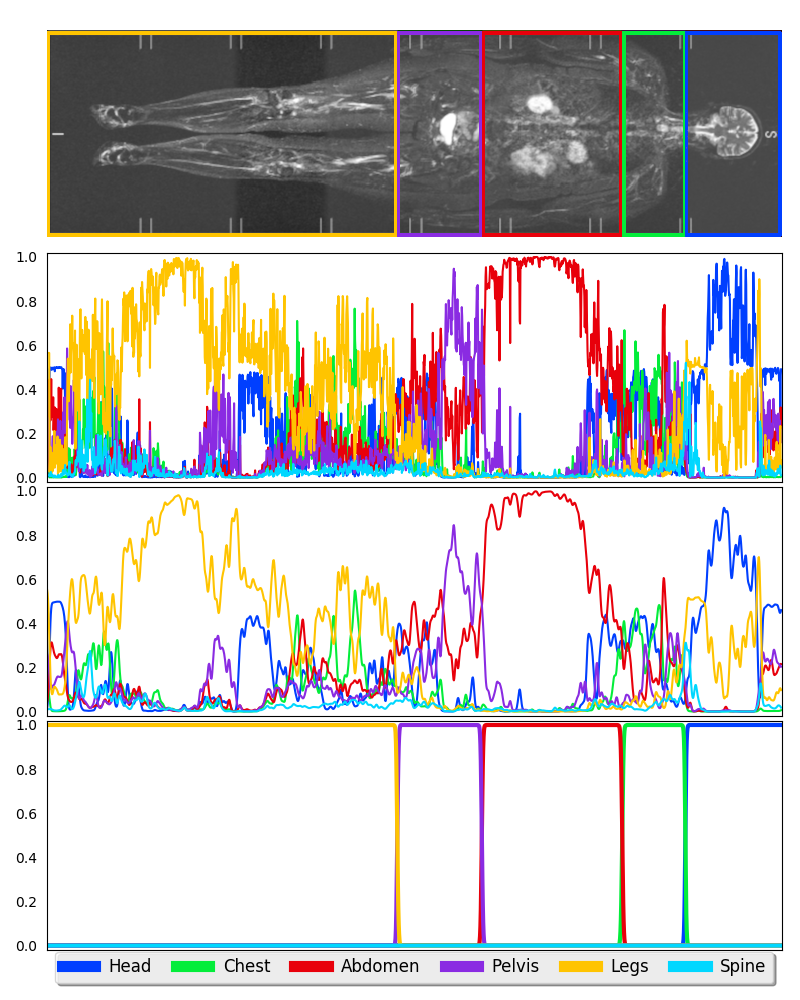
\includegraphics[width=\linewidth]{img_hyperopt/fullbody}
	\caption{\textcolor{red}{CURVES DON'T MATCH IMAGE, TO BE FIXED} Slice by slice prediction on a full body volume. (a) Image and ground truth. (b) Raw model prediction. (c) After smoothing. (d) After selecting the best transitions.}
	\label{fig:full_body}
\end{figure}

Even though we made the choice of processing the data at the slice level, the slices form volumes and we are interested in a decision at the volume level. The first question is: does the model classifies two successive slices similarly ? This is expected since successive slices are anatomically close and have a similar structure. If the model gives very different predictions, this could be a sign that it relies on noise patterns instead of the anatomical structures.

To answer this question, we processed a full body volume by classifying each of its slices through our best model. 
%For each slice, the predicted class is the one with a probability higher than $0.7$, and if no class meets this criterion, then we do not choose any. 
As we can see in Figure~\ref{fig:full_body}, the network is able to identify all body parts, despite the slices being processed independently. Nevertheless the network tends to misclassify the boundaries between regions, notably legs/pelvis and pelvis/abdomen. It also mistakenly identifies the empty slices above the head as being pelvis with a high confidence. This might be indicative of overfitting as those slices contain only noise. Interestingly, the straps used to hold the patient down, visible as the bands with high intensity on the extremities and low intensities on the body, trigger the network every time into the pelvis class. This is likely due to the rarity of those straps in the dataset.

But we are not interested in the mere probabilities, we want to take an actual decision. Therefore we need a decision scheme. A very simple one would be a threshold, say $0.7$, over which we consider the slice to be part of the class. However the predictions from the network are too noisy (see Figure~\ref{fig:full_body}-b), and this approach would give regions broken in multiple parts with messy boundaries.

A more robust decision scheme is the following: start by smoothing the probabilities curves with a Gaussian filter, as illustrated in Figure~\ref{fig:full_body}-c. Then, we remark that only certain transitions are valid, i.e. we can go from pelvis to abdomen, but never from pelvis to head.

[TODO finish describing decision scheme]

\subsection{Conclusion}

We have shown how to use Bayesian optimization to the concrete problem of MR FOV classification. The gain in performance between our handcrafted model and the best model clearly shows the value of automating the search of hyper-parameters, even with a limited budget.

The search was vulnerable to all the weaknesses of Bayesian optimization: the process was sequential (only one model trained at a time), we were limited in the hyper-parameters we could use (no conditional hyper-parameters) and the kernel was stationary. As presented in Section~\ref{ssec:nosta}, work has been done on all those limitations and should be incorporated to improve the process. Other search methods could also be used, such as Hyperband (Section~\ref{sec:cap}). 

Another problem encountered is how to deal with models that cannot be trained (because they require too much memory for example). Not putting them in the training set will just let the search pick other similar models, but putting an arbitrarily high value is not ideal either as the Gaussian process will smoothly interpolate to that value, even though there is a discontinuity in that region (a model that can or cannot be trained, it is binary, not a smooth transition).

Regarding the final models, testing at the volume level has shown that the models are robust and can generalize. Still, the neural network was not enough to obtain smooth coherent predictions, and we presented a decision scheme to fix that.

Further work on this problem would involve improving the dataset by adding new volumes, new anatomical regions and defining stricter boundaries between regions. The model could also be improved by using a cyclic learning rate, spatial dropout on the convolutional layers or replacing the fully-connected layers with convolutional layers.

%%%%%%%%%%%%%%%%%%%%%%%%%%%%%%%%%%%%%%%%%%%%%%%%%%%%%%%%%%%%%%%%%%%%%%%%%%%%%%%%%%%%%%%%%%%%%%%
\section{Conclusion}

When to optimize and with which method ?
